\documentclass{article}
% 这里是导言区
%\usepackage{indentfirst}%缩进控制
\usepackage{listings}%插入代码
\usepackage{mcode}
\usepackage{textcomp}
\usepackage{graphicx}%插入图像
\usepackage{epstopdf}
\usepackage{amsmath}
\usepackage{graphicx}
\usepackage{subfigure}
\usepackage{geometry}%设置页边距
\usepackage{amssymb}
\usepackage{float}
\usepackage[level]{datetime} 
\makeatletter
\newcommand{\rmnum}[1]{\romannumeral #1}
\newcommand{\Rmnum}[1]{\expandafter\@slowromancap\romannumeral #1@}
\makeatother
% \renewcommand\thesection{\roman{subsection}}
%\newdateformat{ukdate}{\ordinaldate{\THEDAY} \monthname[\THEMONTH]

\geometry{a4paper,scale=0.75}


\lstset{
tabsize=4, %tab 空格数
frame=shadowbox, %把代码用带有阴影的框圈起来
rulesepcolor=\color{red!20!green!20!blue!20}, %代码块边框为淡青色
keywordstyle=\color{blue!90}\bfseries, %代码关键字的颜色为蓝色, 粗体
showstringspaces=false, %不显示代码字符串中间的空格标记
stringstyle=\ttfamily, %代码字符串的特殊格式
keepspaces=true, %
breakindent=22pt, %
numbers=left, %左侧显示行号
stepnumber=1, %
numberstyle=\tiny, %行号字体用小号
basicstyle=\footnotesize, %
showspaces=false, %
flexiblecolumns=true, %
breaklines=true, %对过长的代码自动换行
breakautoindent=true, %
breakindent=4em, %
aboveskip=1em, %代码块边框
}

\title{Chapter2}
\author{31202008881        \quad \quad \quad
          Bao Ze an}

\begin{document}
\setlength{\parindent}{2em}
\maketitle
\section*{2.1}
What we know is the linear system must obey the superposition property.\\
The input-output description in Fig2.1(a) is :$y=a*u$.\\
Here $a$ is a constant .It is eay to find the system(a) is a linear system.\\
The input-output decription in Fig2.1(b) is:$y=a*u+b$.\\
Here $a$ and $b$ are all constants.Thstify whether the system has the property of additivity
Let:
\[y_1=a*u_1+b.\]
\[y_2=a*u_2+b.\]
then:
\[(y_1+y_2)=a*(u_1+u_2)+2*b\]
so it does not satisfy the property of additivity.therefore,it is a nonlinear system.\\
It is obviously the system in the Fig2.1(c) is a nonliear system.\\
When system(b) introduce $y-y_0$ as the new output,system(c) can be the linear system.\\

\section*{2.2}
Because $g(t)$ is not zero,when $t \leq 0$,so the ideal lowpass filter is not causual and the ideal filter 
can't build in the real world.\\

\section*{2.3}
It is easy to find the system is a linear system.\\
Testify whether the system is time-invariable:\\
Definine the initial time of input $t_0$,system input is $u(t)$,$t \geq t_0$,so it decides the output $y(t)$,$t \geq t_0$ \\
%用begin{equation}与end{equation}结合的时候,会出现公式序号,所以在不是多个公式的情况下,不要用
%\begin{equation}
\[y(t)=\left\{
\begin{aligned}
&u(t)  , &for& \quad t_0 \leq t \leq \alpha \\
&0  , &for& \quad t \geq \alpha
\end{aligned}
\right.\]
%\end{equation}
Shift the initial time to $t_0+T$.Let $t_0+T> \alpha$,and shift the input to $u(t-T)$,$t \geq t_0+T$.\\
The system output is $y'(t)=0$.Suppose that $u(t)$ is not 0,$y'(t)$ is not equal to $y(t-T)$.\\
So,the system is time-invaring.\\
For any time t,the system output y(t) is decided by the current input u(t) exclusively.\\
So,it is a causual time.\\

\section*{2.4}
Let:$y=Hu$\\
Because of causual property:
\[y_{(- \infty,\alpha)}=Hu_{(-\infty,+\infty)}=Hu_{(-\infty,\alpha)}=HP_\alpha u_{(-\infty,+\infty)}\]\\
Thus we have:
\[P_\alpha y=P_\alpha Hu=P_\alpha HP_\alpha u\]
Because$(P_\alpha Hu)(t)=0$ for $t\geq\alpha$,but $(HP_\alpha u)(t)$can be nonzero for $t \geq\alpha$,
Thus $P_\alpha Hu \neq HP_\alpha u$


\section*{2.5}
* If the system is a nonlinear system,for $x(0) \neq 0$ and $x(0)=0$, all three case are not correct.\\
* If the system is a linear system:\\
\indent Superposition property must hold for the input and initial state.\\
\indent if $x(0) \neq 0$:\\
\indent \indent case1:
\[x(0)+x(0)\neq x(0)\]
\indent \indent so case1 statement is not correct.\\
\indent \indent case2:
\[0.5*x(0)+0.5*x(0)=x(0)\]
\indent \indent so case2 statement is correct.\\
\indent \indent case3:
\[x(0)-x(0)=0 \neq x(0)\]
\indent \indent so case3 statement is correct.\\
\indent if $x(0) = 0$:\\
\indent \indent three statement are all correct.\\

\section*{2.6}
Suppose the system input:$u'(t)=\alpha u(t)$,here $a$ is a constant.\\
The system output:
\[y'(t)=\left\{
\begin{aligned}
&\alpha u^2(t)/u(t-1)& if\quad& u(t-1) \neq 0\\
&0&if\quad&u(t-1)=0\\
\end{aligned}
\right.\]
so,$y'(t)=\alpha y(t)$,it satisfies the homogeneity property.\\
Suppose the input:$u'(t)=u_1(t)+u_2(t)$,
The system output:
\[y'(t)=\left\{
\begin{aligned}
&\alpha (u_1(t)+u2(t))^2(t)/(u_1(t-1)+u_2(t-1))& if\quad& u_1(t-1)+u_2(t-1) \neq 0\\
&0&if\quad&u_1(t-1)+u_2(t-1)=0\\
\end{aligned}
\right.\]
in some case,$y'(t) \neq y_1(t)+y_2(t)$,so it don't satisfy the additivity property

\section*{2.7}
Any rational number $\alpha=m/n$,here $m$ and $n$ are both integer.
Firstly,prove that if the system input-output can be decribed as following:
\[x\rightarrow y\]
then:
\[mx\rightarrow my\]\\
The input $mx$ can be regarded as the sum of m input $x$.\\
It is easy to testify it satisfy the additivity.\\
Secondly, prove that if a system input-output can be described as following:
\[x \rightarrow y\]
then:
\[x/n \rightarrow y/n\]
Suppose:%假设将x/n当作输入,而输出的是u
\[x/n\rightarrow u\]
using additivity:
\[n*(x/n)=x\]
thus to say:$n*(x/n)\rightarrow y$,in the same time,from the above statement,$n*(x/n)\rightarrow nu$
so:
\[y=nu\]
\[u=y/n\]
thus:
\[x/n\rightarrow y/n\]
\[x*m/n \rightarrow y*m/n \]
\[\alpha x\rightarrow \alpha y\]

\section*{2.8}
Define:
\[x=t+\tau y=t-\tau\]
so:
\[t=\frac{x+y}{2} \tau=\frac{x-y}{2}\]
for all $t,\tau$:

\[
\begin{aligned}
g(t,\tau)&=g(\frac{x+y}{2},\frac{x-y}{2})\\
&=g(\frac{x+y}{2}+\frac{-x+y}{2},\frac{x-y}{2}+\frac{-x+y}{2})\\
&=g(y,0)\\   
\end{aligned}\]
so:
\[\frac{\partial g(t,\tau)}{\partial x}=\frac{\partial g(y,0)}{\partial x}=0\]
it just prove the $g(t,\tau)$ depends only on the $t-\tau.$

\section*{2.9}
\subsection*{\rmnum{1}}when $t<0,y(t)=0$\\
\subsection*{\rmnum{2}}when $0 \leq t \leq 1$
\[y(t)=\int_{0}^{t} g(t-\tau)u(\tau) d\tau\]
take the convolution integral:
\par
\centerline{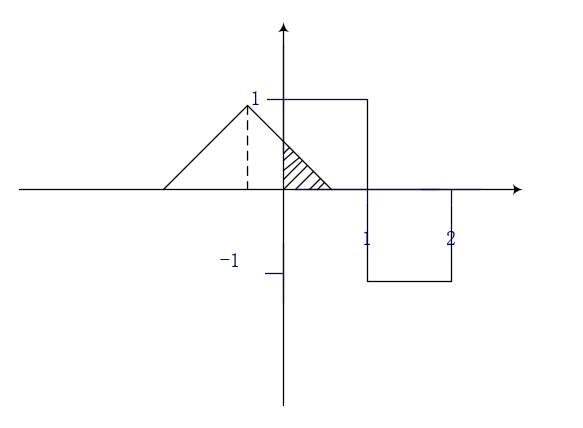
\includegraphics[width = .8\textwidth]{a2.9_1.PNG}}
\centerline
\par
\[y(t)=\int_{0}^{t}(t-\tau)d\tau\]
\[y(t)=\frac{1}{2}t^2\]
\subsection*{\rmnum{3}} when $ 1<t \leq 2$
take the convolution integral:
\par
\centerline{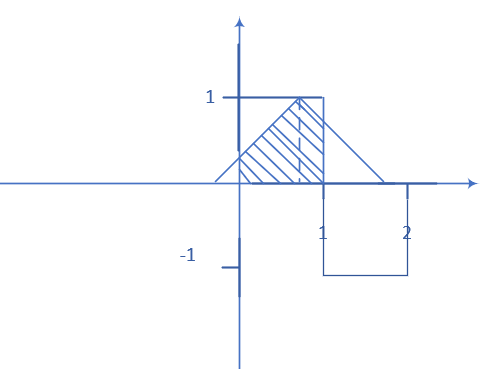
\includegraphics[width = .8\textwidth]{a2.9_2.PNG}}
\centerline
\par
\[y(t)=1-\frac{(2-t)^2}{2}-\frac{(t-1)^2}{2}\]
the image on full definition domain:
\par
\centerline{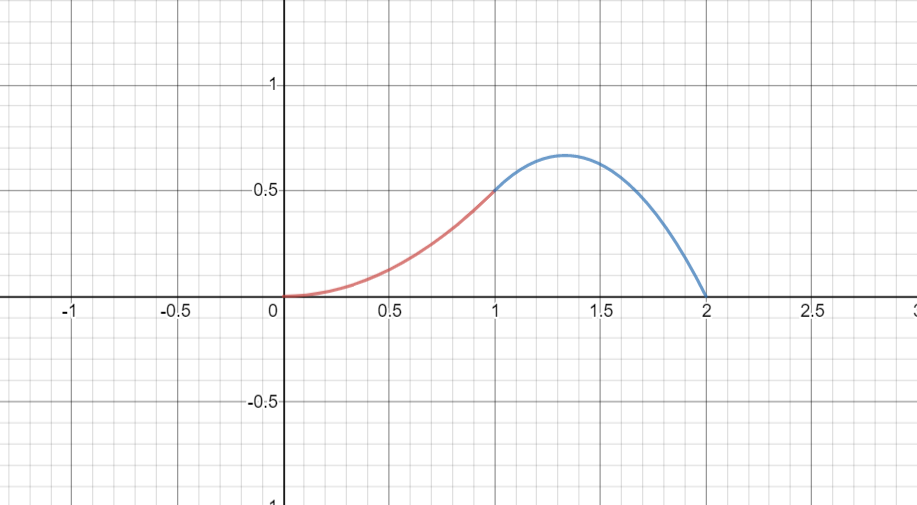
\includegraphics[width = .8\textwidth]{a2.9_3.PNG}}
\centerline
\par

\section*{2.10}
\subsection*{\rmnum{1}}
Take the lapalace transform to both sides of the equation:
\[s^2\hat{y(s)}+2s\hat{y(s)}-3\hat{y(s)}=s\hat{u(s)}-\hat{u(s)}\]
arrange the equation:
\[g(s)=\frac{\hat{y(s)}}{\hat{u(s)}}=\frac{s-1}{s^2+2s-3}=\frac{1}{s+3}\]
the impulse response of the system is just the inverse lapalace 
%花体拉氏变换字母\mathcal{L}
\[g(t)= \mathcal{L}^{-1}[\hat{g(s)}]=e^{-3t} \quad\quad\quad\quad t \geq 0\]

\section*{2.11}
Let g(t) is the impulse response,u(t)=1 is the input.so the unit-step response is:
\[\overline{y}(t)=\int_{0}^{t}g(t)u(t-\tau)d\tau=\int_{0}^{t}g(\tau)d\tau\]
Therefore g(t)=$\frac{\mathrm{d}\overline{y}(t)}{\mathrm{d}t}$

\section*{2.12}
Take the lapalace transform to both sides of the equations:
\[D_{11}(s)y_1(s)+D_{12}(s)y_2(s)=N_{11}(s)u_1(s)+N_{12}(s)u_2(s)\]
\[D_{21}(s)y_1(s)+D_{22}(s)y_2(s)=N_{21}(s)u_1(s)+N_{22}(s)u_2(s)\]
Rewrite them in matrix form:
\begin{equation*}       %开始数学环境
\left[                %左括号
\begin{array}{cc}   %该矩阵一共3列,每一列都居中放置
D_{11}(s) & D_{12}(s) \\  %第一行元素
D_{21}(s) & D_{22}(s) \\  %第二行元素
\end{array}
\right]      %右括号
\left[                %左括号
\begin{array}{c}   %该矩阵一共3列,每一列都居中放置
y_1(s) \\  %第一行元素
y_2(s) \\  %第二行元素
\end{array}
\right]=
\left[                %左括号
\begin{array}{cc}   %该矩阵一共3列,每一列都居中放置
N_{11}(s) & N_{12}(s) \\  %第一行元素
N_{21}(s) & N_{22}(s) \\  %第二行元素
\end{array}
\right]
\left[                %左括号
\begin{array}{c}   %该矩阵一共3列,每一列都居中放置
u_1(s) \\  %第一行元素
u_2(s) \\  %第二行元素
\end{array}
\right]                  
\end{equation*}
so the transfer matrix of the system is:
\begin{equation*}
\hat{G}(s)=\left[                %左括号
\begin{array}{cc}   %该矩阵一共3列,每一列都居中放置
D_{11}(s) & D_{12}(s) \\  %第一行元素
D_{21}(s) & D_{22}(s) \\  %第二行元素
\end{array}
\right]^{-1}      %右括号
\left[                %左括号
\begin{array}{cc}   %该矩阵一共3列,每一列都居中放置
N_{11}(s) & N_{12}(s) \\  %第一行元素
N_{21}(s) & N_{22}(s) \\  %第二行元素
\end{array}
\right]
\end{equation*}

\section*{2.13}
%[htbp]参数的作用可以用来控制图片的位置
\begin{figure}[htbp]
\begin{minipage}[t]{0.5\linewidth} 
\centering 
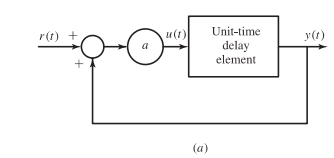
\includegraphics{a2.132.PNG} 
\caption{system with negative feedback} 
\label{frame} 
\end{minipage}% 
\begin{minipage}[t]{0.5\linewidth} 
\centering 
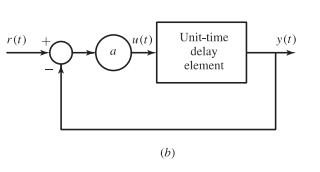
\includegraphics{a2.131.PNG} 
\caption{system with positive feedback} 
\label{label} 
\end{minipage} 
\end{figure}
\subsection*{\rmnum{1}:the positive feedback system}
\[y(t)=u(t-1),r(t)=1 \quad\quad\quad\quad for\quad t \geq 0\]
$a=1:$\\
\[u(t)=r(t)+y(t)=1+u(t-1)\]
thus to say:
\[y(t+1)=1+y(t)\]
From the initial condition:$y(t)=0$ for $0 \leq t <1$,then:\\
\[y(t)=1 \quad\quad for \quad 1 \leq t <2 \]
\[y(t)=2 \quad\quad for \quad  2 \leq t <3 \]
\[\vdots\]

\[y(t)=n \quad\quad for \quad n \leq t <(n+1) \]
so the image of the y(t):
\par
\centerline{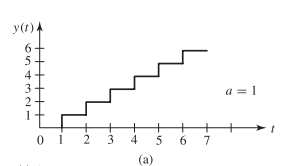
\includegraphics{a2.133.PNG}}
\centerline
\par

$a=0.5:$\\
\[u(t)=0.5(r(t)+y(t))=0.5+0.5y(t)\]
thus to say:
\[y(t+1)=0.5+0.5y(t)\]
From the initial condition:$y(t)=0$ for $0 \leq t <1$,then:\\
\[y(t)=0.5 \quad\quad for \quad 1 \leq t <2 \]
\[y(t)=0.75 \quad\quad for \quad  2 \leq t <3 \]
\[\vdots\]
so the image of the y(t):
\par
\centerline{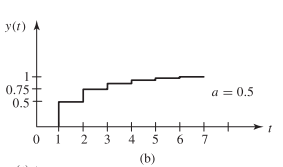
\includegraphics{a2.134.PNG}}
\centerline
\par

\subsection*{\rmnum{2}:the negative feedback system}
\[y(t)=u(t-1),r(t)=1 \quad\quad\quad\quad for\quad t \geq 0\]
$a=1:$
\[u(t)=r(t)-y(t)=1-u(t-1)\]
thus to say:
\[y(t+1)=1-y(t)\]
From the initial condition:$y(t)=0$ for $0 \leq t <1$,then:\\
\[y(t)=1 \quad\quad for \quad 1 \leq t <2 \]
\[y(t)=0 \quad\quad for \quad  2 \leq t <3 \]
\[y(t)=1 \quad\quad for \quad  3 \leq t <4 \]
\[\vdots\]
so the image of the y(t):
\par
\centerline{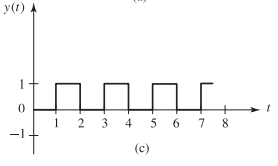
\includegraphics{a2.135.PNG}}
\centerline
\par

$a=0.5:$
\[u(t)=0.5(r(t)-y(t))=0.5-0.5u(t-1)\]
thus to say:
\[y(t+1)=0.5-0.5y(t)\]
From the initial condition:$y(t)=0$ for $0 \leq t <1$,then:\\
\[y(t)=0.5 \quad\quad for \quad 1 \leq t <2 \]
\[y(t)=0.25 \quad\quad for \quad  2 \leq t <3 \]
\[y(t)=0.375 \quad\quad for \quad  3 \leq t <4 \]
\[\vdots\]
so the image of the y(t):
\par
\centerline{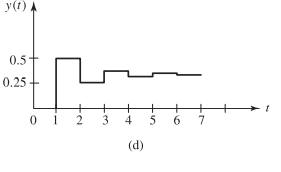
\includegraphics{a2.136.PNG}}
\centerline
\par

\section*{2.14}
From the state-space equation,it has 2 dimensions,,so we need two intergerators to implement it.\\
We choose the output of number 1 intergerators as $+x_2$,and the output of number 2 intergerators as $-x_1$.\\
We suppose $RC=1$:\\
The op-amp circuit diagram:\\
\par
\centerline{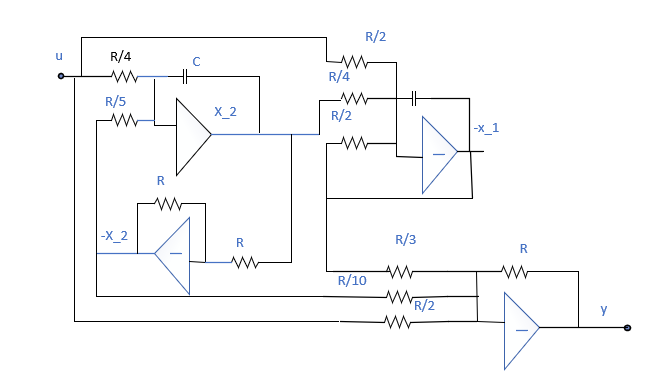
\includegraphics{a2.141.PNG}}
\centerline
\par

\section*{2.15}
\subsection*{a}
Application of Newton's law to the rotaional movement of the pendulum:\\
Moment of gravity component to pendulum:$M=(ucos\theta-mgsin\theta)l$\\
According to the angular momentum theorem:\\
\[M=I\beta=ml^2\frac{\mathrm{d}^2 \theta}{\mathrm{d}t^2}\]
thus to say:
\[ml^2\frac{\mathrm{d}^2 \theta}{\mathrm{d}t^2}=(ucos\theta-mgsin\theta)l\]
choose the $\dot{\theta},\theta$ as the state variable
Define $x_1=\theta,x_2=\dot{\theta}$
%\sim是波浪号
\[\left\{
\begin{aligned}
&\dot{x_1}=x_2&\\
&\dot{x_2}=-\frac{g}{l}sinx_1+\frac{u}{ml}cosx_1&\\
\end{aligned}
\right.\]
The system is nonlinear.
If $\theta$ is very small:$sin\theta \sim \theta,cos\theta \sim 1$
so the state-space equation is:
\begin{equation*}       %开始数学环境
\left[                %左括号
\begin{array}{c}   %该矩阵一共3列,每一列都居中放置
\dot{x_1} \\  %第一行元素
\dot{x_2} \\  %第二行元素
\end{array}
\right]=      %右括号
\left[                %左括号
\begin{array}{cc}   %该矩阵一共3列,每一列都居中放置
0 & 1 \\  %第一行元素
-\frac{g}{l} & 0 \\  %第二行元素
\end{array}
\right]
\left[                %左括号
\begin{array}{c}   %该矩阵一共3列,每一列都居中放置
x_1 \\  %第一行元素
x_2 \\  %第二行元素
\end{array}
\right]+
\left[                %左括号
\begin{array}{c}   %该矩阵一共3列,每一列都居中放置
0 \\  %第一行元素
\frac{1}{ml}\\  %第二行元素
\end{array}
\right]u                
\end{equation*}
when $\theta$ is very small, we can consider the system is linear.

\subsection*{b}
In the same way:\\
for $m_2$ and $l_2$:
\[m_2l_2^2 \frac{\mathrm{d}^2 \theta_2}{\mathrm{d}t^2}=(ucos\theta_2-m_2gsin\theta_2)l_2\]
for $m_1$ and $l_1$,define the force on the $l_2$ is $T$:\\
\[T=m_2gcos\theta_2+usin\theta_2\]
\[m_1l_1^2\frac{\mathrm{d}^2 \theta_1}{\mathrm{d}t^2}=(-m_1gsin\theta_1+Tsin(\theta_2-\theta_1))l_1\]
Define $x_1=\theta_1,x_2=\dot{\theta_1},x_3=\theta_2,x_4=\dot{\theta_2}$
\[\left\{
\begin{aligned}
&\dot{x_1}=x_2&\\
&\dot{x_2}=-\frac{g}{l_1}sinx_1+\frac{m_2gcosx_3sin(x_3-x_1)}{m_1l_1}+\frac{usinx_3sin(x_3-x_1)}{m_1l_1}&\\
&\dot{x_3}=x_4&\\
&\dot{x_4}=-\frac{gsinx_3}{l_2}+\frac{ucosx_3}{m_2l_2}&\\
\end{aligned}
\right.\]
The system is nonlinear.
If $\theta$ is very small:$sin\theta_1 \sim \theta_1,sin\theta_2 \sim \theta_2,cos\theta_1 \sim 1,cos\theta_2 \sim 1$
so the state-space equation is:
\begin{equation*}       %开始数学环境
\left[                %左括号
\begin{array}{c}   %该矩阵一共3列,每一列都居中放置
\dot{x_1} \\  %第一行元素
\dot{x_2} \\  %第二行元素
\dot{x_3} \\
\dot{x_4} \\
\end{array}
\right]=      %右括号
\left[                %左括号
\begin{array}{cccc}   %该矩阵一共3列,每一列都居中放置
0 & 1 & 0 &0\\  %第一行元素
-\frac{g}{l_1}-\frac{m_1g}{m_1l_1} & 0 &\frac{m_2g}{m_1l_1} & 0 \\  %第二行元素
0 & 0 & 0 &1\\
0 & 0 & -\frac{g}{l_2} & 0\\
\end{array}
\right]
\left[                %左括号
\begin{array}{c}   %该矩阵一共3列,每一列都居中放置
x_1 \\  %第一行元素
x_2 \\  %第二行元素
x_3 \\
x_4 \\
\end{array}
\right]+
\left[                %左括号
\begin{array}{c}   %该矩阵一共3列,每一列都居中放置
0 \\  %第一行元素
0 \\  %第二行元素
0 \\
\frac{1}{m_2l_2}\\
\end{array}
\right]u                
\end{equation*}
when $\theta_1,\theta_2$ is very small, we can consider the system is linear.

\section*{2.16}
According to Newton's second law,we can get the equation:\\
\[m\ddot{h}=f_1-f_2=k_1\theta-k_2u\]
According to the angular momentum theorem,we can get the equation:
\[I\ddot{\theta}+b\dot{\theta}=(l_1+l_2)f_2-l_1f_1\]
Define $x_1=h,x_2=\dot{h},x_3=\theta,x_4=\dot{\theta}:$
\[\left\{
\begin{aligned}
&\dot{x_1}=x_2&\\ 
&\dot{x_2}=\frac{k_1}{m}x_3-\frac{k_2}{m}u&\\
&\dot{x_3}=x_4&\\  
&\dot{x_4}=-\frac{l_1k_1}{I}x_3-\frac{b}{I}x_4+\frac{(l_1+l_2)k_2}{I}u&\\
\end{aligned}
%下面的.号不是可有可无的,是必须有的,可以理解为一种分隔符
\right.
\]
If neglecting the effect of I,two equations became:\\
\[m\ddot{h}=f_1-f_2=k_1\theta-k_2u\]
\[b\dot{\theta}=(l_1+l_2)f_2-l_1f_1\]
Simultaneous equations,take Lapalace transform to both sides of equations, eliminating variable $\theta$\\
\[ms^2h(s)=k_1\theta(s)-k_2u(s)\]
\[bs\theta(s)=(l_1+l_2)k_2u(s)-l_1k_1\theta(s)\]
so,the transfer function from u to h is:
\[\hat{g}(s)=\frac{\hat{h}(s)}{\hat{u}(s)}=\frac{k_1k_2l_2-k_2bs}{ms^2(bs+k_1l_1)}\]

\section*{2.17}
%这道题给我的反思是不要老想着矩阵的那种形式,只要和相应的状态变量相关即可,
%这是非线性的一种状态
A state-space equation to describe the system is:\\
\[\left\{
\begin{aligned}
&\dot{x}_1=x_2&\\
&\dot{x}_2=-\frac{k}{m}x_3-g&\\
&\dot{x}_3=u&\\
\end{aligned}
\right.
\]

\section*{2.18}
Refer to example 2.9, we can get the equations following:\\
\[y_1=\frac{x_1}{R_1}\quad and \quad y_2=\frac{x_2}{R_2} \]
Changes of liquid levels are governed by:
\[A_1dx_1=(u-y_1)dt\]
\[A_2dx_2=(y-y_1)dt\]
Thus to say:
\[\left\{
\begin{aligned}
&A_1\dot{x_1}=u-\frac{x_1}{R_1}&\\
&A_2\dot{x_2}=\frac{x_1}{R_1}-\frac{x_2}{R_2}&\\
\end{aligned} 
\right.
\]
Take the lapalace transform:
\[\frac{\hat{y}_1(s)}{\hat{u}(s)}=\frac{1}{A_1R_1s+1}\]

the transfer function from $y_1$ to y:\\
\[\frac{\hat{y}(s)}{\hat{y}_1(s)}=\frac{1}{A_2R_2s+1}\]

the transfer function from u to y:\\
\[\frac{\hat{y}(s)}{\hat{u}(s)}=\frac{1}{(A_1R_1s+1)(A_2R_2s+1)}\]
So the transfer function from u to y equal the product of the two transfer functions.\\

\section*{2.19}
%一定要注意电路里的源是电流源还是电压源
%这对树(tree)的选取至关重要。
\par
\centerline{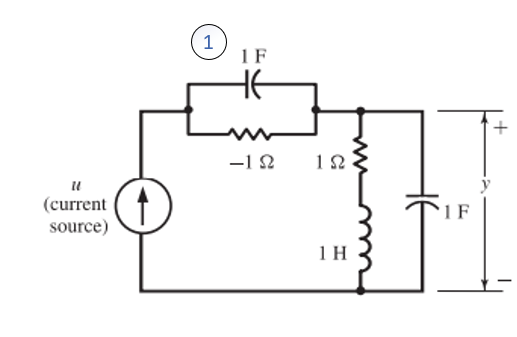
\includegraphics{a2.191.PNG}}
\centerline
\par
The voltage across the 1-F capacitor number 1 is assigned $x_1$,then its current is $\hat{x_1}$,the voltage across the other 1-F capacitor is assigned
$x_2$,then its current is $\hat{x_2}$,the current through the 1-H inductor is assigned as $x_3$,
then its voltage is $\hat{x_3}$\\
According to the Kirchhoff's current law and Kirchhoff's voltage law,we can get the equation following:
\[\left\{    
\begin{aligned}
&\dot{x_1}=x_1+u&\\
&\dot{x_2}=-x_3+u&\\
&\dot{x_3}=x_2-x_3&\\
&y=x_2&\\
\end{aligned}
\right.
\]
Rewrite them in matrix form:
\begin{equation*}       %开始数学环境
    \left[                %左括号
    \begin{array}{c}   %该矩阵一共3列,每一列都居中放置
    \dot{x_1} \\  %第一行元素
    \dot{x_2} \\  %第二行元素
    \dot{x_3} \\
    \end{array}
    \right]=      %右括号
    \left[                %左括号
    \begin{array}{ccc}   %该矩阵一共3列,每一列都居中放置
    -1 & 0 & 0\\
    0 & 0 & -1\\
    0 & 1 & -1\\    
    \end{array}
    \right]
    \left[                %左括号
    \begin{array}{c}   %该矩阵一共3列,每一列都居中放置
    x_1 \\  %第一行元素
    x_2 \\  %第二行元素
    x_3 \\
    \end{array}
    \right]+
    \left[                %左括号
    \begin{array}{c}   %该矩阵一共3列,每一列都居中放置
    1 \\  %第一行元素
    1 \\  %第二行元素
    0 \\
    \end{array}
    \right]u               
\end{equation*}

\begin{equation*}
y=\left[
\begin{array}{ccc}
0 & 1 & 0\\
\end{array}
\right]
\left[
\begin{array}{c}
x_1 \\  %第一行元素
x_2 \\  %第二行元素
x_3 \\
\end{array}
\right]
\end{equation*}


Its transfer matrix from the state-space equation:\\
\[\hat{g}(s)=\frac{\hat{y}(s)}{\hat{u}(s)}=C(SI-A)^{-1}B=\frac{s+1}{s^2+s+1}\]

\section*{2.20}
\par
\centerline{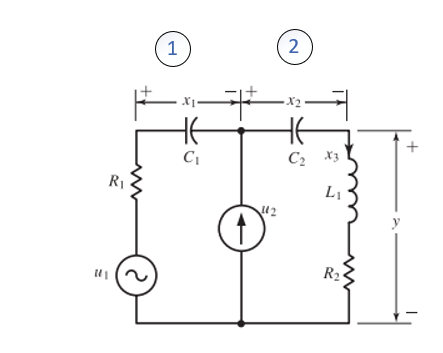
\includegraphics{a2.192.PNG}}
\centerline
\par
Select the state variable as shown in the figure,According to the Kirchhoff's current law and Kirchhoff's voltage law,we can get the equation following:\\
\[\left\{    
\begin{aligned}
&C_1\dot{x_1}=x_3-u_2&\\
&C_2\dot{x_2}=x_3&\\
&L_1\dot{x_3}=u_1-x_1-x_2-R_2x_3-C_1\dot{x_1}R_1&\\
&y=u_1-C_1\dot{x_1}R_1-x_1-x_2&\\
\end{aligned}
\right.
\]
Rewrite them in matrix form:
\begin{equation*}       %开始数学环境
    \left[                %左括号
    \begin{array}{c}   %该矩阵一共3列,每一列都居中放置
    \dot{x_1} \\  %第一行元素
    \dot{x_2} \\  %第二行元素
    \dot{x_3} \\
    \end{array}
    \right]=      %右括号
    \left[                %左括号
    \begin{array}{ccc}   %该矩阵一共3列,每一列都居中放置
    0 & 0 & \frac{1}{C_1}\\
    0 & 0 & \frac{1}{C_2}\\
    -\frac{1}{L_1} & -\frac{1}{L_1} & -\frac{R_1+R_2}{L_1}\\    
    \end{array}
    \right]
    \left[                %左括号
    \begin{array}{c}   %该矩阵一共3列,每一列都居中放置
    x_1 \\  %第一行元素
    x_2 \\  %第二行元素
    x_3 \\
    \end{array}
    \right]+
    \left[                %左括号
    \begin{array}{cc}   %该矩阵一共3列,每一列都居中放置
    0 & -\frac{1}{C_1} \\  %第一行元素
    0 & 0 \\  %第二行元素
    \frac{1}{L_1} & \frac{R_1}{L_1} \\
    \end{array}
    \right]
    \left[                %左括号
    \begin{array}{c}   %该矩阵一共3列,每一列都居中放置
    u_1 \\  %第一行元素
    u_2 \\  %第二行元素
    \end{array}
    \right]               
\end{equation*}

\begin{equation*}
    y=\left[
    \begin{array}{ccc}
    -1 & -1 & -R_1\\
    \end{array}
    \right]
    \left[
    \begin{array}{c}
    x_1 \\  %第一行元素
    x_2 \\  %第二行元素
    x_3 \\
    \end{array}
    \right]+
    \left[
    \begin{array}{cc}
    1 & R_1\\  %第一行元素
    \end{array}
    \right]
    \left[
    \begin{array}{c}
    u_1 \\  %第一行元素
    u_2 \\  %第二行元素
    \end{array}
    \right]
    \end{equation*}

It is a two-input one-output system,So its transfer function matrix is 2x1 dimension.
\subsection*{\rmnum{1}: The transfer function from $u_1$ to y}
Let the $u_2$=0,the components are expressed in the form of complex impedance,we can get the equation:\\
\par
\centerline{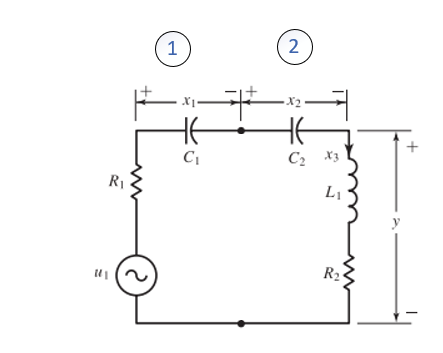
\includegraphics{a2.201.PNG}}
\centerline
\par
\[\hat{g}_1(s)=\frac{L_1s+R_2}{R_1+\frac{1}{C_1s}+\frac{1}{C_2s}+L_1s+R_2}=\frac{s^2+\frac{R_2}{L_1}s}{s^2+\frac{R_1+R_2}{L_1}s+\frac{C_1+C_2}{C_1C_2L_1}}\]

\subsection*{\rmnum{1}: The transfer function from $u_2$ to y}
In the same way:
\par
\centerline{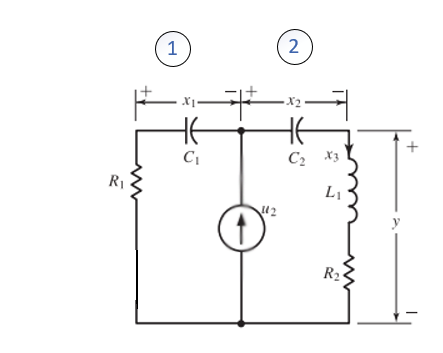
\includegraphics{a2.202.PNG}}
\centerline
\par
According to the shunt formula:
the current through $L_1$:
\[\hat{i}(s)=\frac{\frac{1}{C_1s}+R_1}{R_1+R_2+\frac{1}{C_1s}+\frac{1}{C_2s}+L_1s}\hat{u_2}(s)\]
\[\hat{y}(s)=(L_1s+R_1)\hat{i}(s)\]
so:
\[\hat{g}_2(s)=\frac{\hat{y}(s)}{\hat{u}_2(s)}=\frac{(\frac{1}{C_1s}+R_1)(L_1s+R_2)}{R_1+R_2+\frac{1}{C_1s}+\frac{1}{C_2s}+L_1s}\]
The ultimate transfer function matrix:\\
\[\hat{G}(s)=[\hat{g}_1(s)\quad \quad  \hat{g}_2(s)]\]

\section*{2.21}
Neglecting the mass of $m_1$ and $m_2$\\
If the $\theta$ is very small,according to Newton's second law and the angular momentum theorem:
\[m_2\ddot{y}=k_2(l_2\theta-y)\]
\[I\ddot{\theta}=ul_2-k_1(l_1\theta)l_1-k_2(l_2\theta-y)l_2\]
Define $x_1=\theta,x_2=\dot{\theta},x_3=y,x_4=\dot{y}$
Rewrite them in matrix form:

\begin{equation*}       %开始数学环境
    \left[                %左括号
    \begin{array}{c}   %该矩阵一共3列,每一列都居中放置
    \dot{x_1} \\  %第一行元素
    \dot{x_2} \\  %第二行元素
    \dot{x_3} \\\
    \dot{x_4} \\
    \end{array}
    \right]=      %右括号
    \left[                %左括号
    \begin{array}{cccc}   %该矩阵一共3列,每一列都居中放置
    0 & 1 & 0 & 0\\
    -\frac{(k_1l_1^2+k_2l_2^2)}{I} & 0 & \frac{k_2l_2}{I} & 0\\
    0 & 0 & 0 & 1\\
    \frac{k_2l_2}{m_2} & 0 & -\frac{k_2}{m_2} & 0\\    
    \end{array}
    \right]
    \left[                %左括号
    \begin{array}{c}   %该矩阵一共3列,每一列都居中放置
    x_1 \\  %第一行元素
    x_2 \\  %第二行元素
    x_3 \\
    x_4 \\
    \end{array}
    \right]+
    \left[                %左括号
    \begin{array}{c}   %该矩阵一共3列,每一列都居中放置
    0\\
    \frac{l_2}{I}\\
    0\\
    0\\
    \end{array}
    \right]u               
\end{equation*}

\begin{equation*}
    y=\left[
    \begin{array}{cccc}
    0 & 0 & 1 & 0\\
    \end{array}
    \right]
    \left[
    \begin{array}{c}
    x_1 \\  %第一行元素
    x_2 \\  %第二行元素
    x_3 \\
    x_4
    \end{array}
    \right]
    \end{equation*}


Take the lapalace transform to both sides of equations:
\[m_2s^2\hat{y}(s)=k_2l_2\theta(s)-k_2\hat{y}(s)\]
\[Is^2\hat{\theta}(s)=\hat{u}(s)l_2-k_1l_1^2\hat{\theta}(s)-k_2l_2^2\hat{\theta}(s)+k_2l_2\hat{y}(s)\]
arrange them:
\[\hat{g}(s)=\frac{\hat{y}(s)}{\hat{u}(s)}=\frac{k_2l_2^2}{m_2Is^4+(k_2I+(k_1l_1^2+k_2l_2^2)m_2)s^2+k_1k_2l_1^2}\]

\[g(s)=C(sI-A)^{-1}B+E\]
\end{document}



